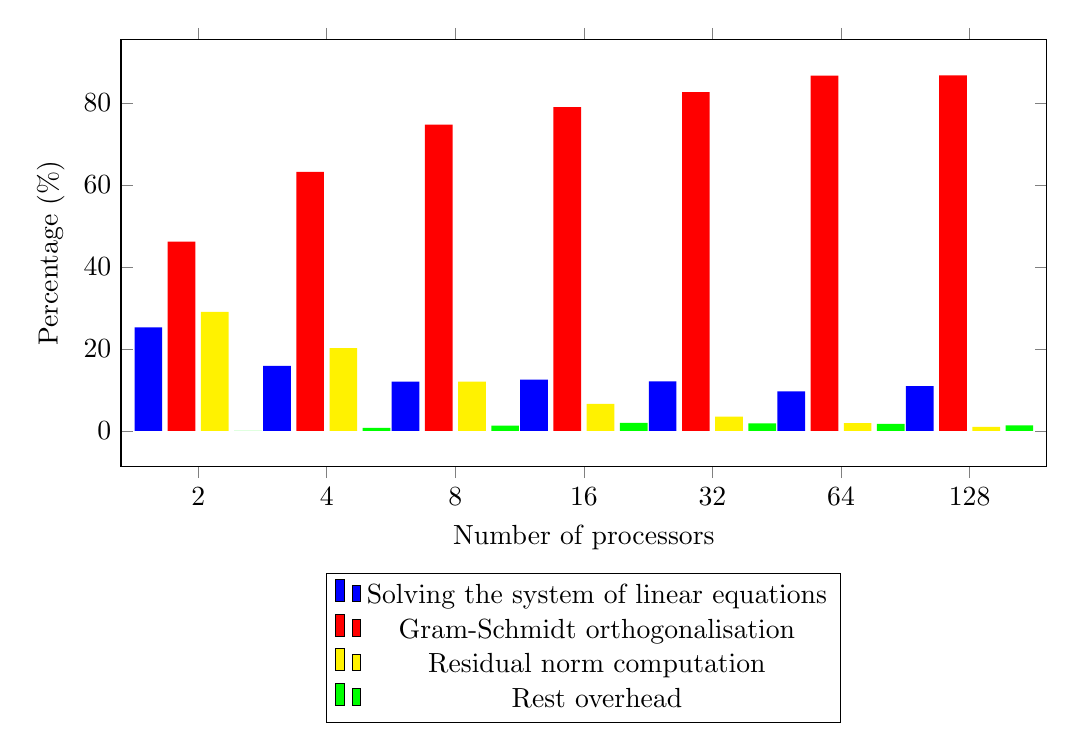
\begin{tikzpicture}
 \begin{axis}[
  ybar,
  height=7cm,
  width=1.1\textwidth,
  xlabel=Number of processors,
  xtick={0, 1, 2, 3, 4, 5, 6},
  xticklabels={2, 4, 8, 16, 32, 64, 128},
  legend style={
   at={(0.5, -0.25)},
   anchor=north
  },
  ylabel={Percentage (\%)}]
  \addplot[draw=none, fill=blue] coordinates {
   (0, 25.27)
   (1, 15.88)
   (2, 12.04)
   (3, 12.49)
   (4, 12.08)
   (5, 9.64)
   (6, 10.91)};
  \addplot[draw=none, fill=red] coordinates {
   (0, 46.15)
   (1, 63.20)
   (2, 74.71)
   (3, 79)
   (4, 82.65)
   (5, 86.71)
   (6, 86.76)};
  \addplot[draw=none, fill=yellow] coordinates {
   (0, 29.05)
   (1, 20.17)
   (2, 12.01)
   (3, 6.58)
   (4, 3.46)
   (5, 1.92)
   (6, 0.97)};
  \addplot[draw=none, fill=green] coordinates {
   (0, 0)
   (1, 0.75)
   (2, 1.25)
   (3, 1.93)
   (4, 1.81)
   (5, 1.73)
   (6, 1.37)};
  \legend{
   Solving the system of linear equations,
   Gram-Schmidt orthogonalisation,
   Residual norm computation,
   Rest overhead}
 \end{axis}
\end{tikzpicture}
